\documentclass[a4paper, 10pt, ]{article}

\usepackage[slovak]{babel}

% ------------------------------

\usepackage[utf8]{inputenc}
\usepackage[T1]{fontenc}

\usepackage[left=4cm,
			right=4cm,
			top=2.1cm,
			bottom=2.6cm,
			footskip=7.5mm,
			twoside,
			marginparwidth=3.0cm,
			%showframe,
			]{geometry}

\usepackage{graphicx}
\usepackage[dvipsnames]{xcolor}
% https://en.wikibooks.org/wiki/LaTeX/Colors

% ------------------------------

\usepackage{lmodern}

\usepackage[tt={oldstyle=false,proportional=true,monowidth}]{cfr-lm}
% https://mirror.szerverem.hu/ctan/fonts/cfr-lm/doc/cfr-lm.pdf

% ------------------------------

\usepackage{amsmath}
\usepackage{amssymb}
\usepackage{amsthm}

\usepackage{booktabs}
\usepackage{multirow}
\usepackage{array}
\usepackage{dcolumn}

% \usepackage{natbib}





% ------------------------------

\hyphenpenalty=6000
\tolerance=1000

\def\naT{\mathsf{T}}

% ------------------------------

\makeatletter

	\def\@seccntformat#1{\protect\makebox[0pt][r]{\csname the#1\endcsname\hspace{4mm}}}

	\def\cleardoublepage{\clearpage\if@twoside \ifodd\c@page\else
	\hbox{}
	\vspace*{\fill}
	\begin{center}
	\phantom{}
	\end{center}
	\vspace{\fill}
	\thispagestyle{empty}
	\newpage
	\if@twocolumn\hbox{}\newpage\fi\fi\fi}

	\newcommand\figcaption{\def\@captype{figure}\caption}
	\newcommand\tabcaption{\def\@captype{table}\caption}

\makeatother

% ------------------------------

\usepackage{fancyhdr}
\fancypagestyle{plain}{%
\fancyhf{} % clear all header and footer fields
% \fancyfoot[C]{\sffamily {\bfseries \thepage}\ | {\scriptsize\oznacenieCasti}}
\fancyfoot[C]{\sffamily {\bfseries \thepage}{\color{Gray}\scriptsize$\,$z$\,$\pageref{LastPage}}\ | \includegraphics[height=5pt]{../../KUT000/KUT_logo_v0.1.pdf}{\scriptsize\KUTporadoveCislo}}
\renewcommand{\headrulewidth}{0pt}
\renewcommand{\footrulewidth}{0pt}}
\pagestyle{plain}

% ------------------------------

\usepackage{titlesec}
\titleformat{\paragraph}[hang]{\sffamily  \bfseries}{}{0pt}{}
\titlespacing*{\paragraph}{0mm}{3mm}{1mm}
\titlespacing*{\subparagraph}{0mm}{3mm}{1mm}

\titleformat*{\section}{\sffamily\Large\bfseries}
\titleformat*{\subsection}{\sffamily\large\bfseries}
\titleformat*{\subsubsection}{\sffamily\normalsize\bfseries}


% ------------------------------

\PassOptionsToPackage{hyphens}{url}
\usepackage[pdfauthor={},
			pdftitle={},
			pdfsubject={},
			pdfkeywords={},
			% hidelinks,
			colorlinks=false,
			breaklinks,
			]{hyperref}


% ------------------------------

\graphicspath{%
{./COMMONFILES/}%
{../SVG/}%
{../PY/fig/}%
{../PY/jupynotex/fig/}%
{../ML/fig/}%
}

% ------------------------------

\usepackage{enumitem}

\usepackage{lettrine}

% ------------------------------

\usepackage{lastpage}

\usepackage{microtype}

% ------------------------------

% \usepackage[backend=biber,
%             style=numeric,
%             sorting=none,
%             ]{biblatex}
% \DeclareSourcemap{
%     \maps[datatype=bibtex]{
%         \map{
%         \step[fieldset=note, null]
%         }
%         \map{
%         \step[fieldset=file, null]
%         }        
%         % \map{
%         % \step[fieldset=url, null]        
%         % }
%         \map{
%         \step[fieldset=eprint, null]
%         }
%     }
% }
% 
% \addbibresource{./COMMONFILES/biblist.bib}



% ------------------------------



\usepackage{listings}




\renewcommand{\lstlistingname}{Výpis kódu}
\renewcommand{\lstlistlistingname}{Výpisy kódu}


%New colors defined below
\definecolor{codegreen}{rgb}{0,0.6,0}
\definecolor{codegray}{rgb}{0.5,0.5,0.5}
\definecolor{codepurple}{rgb}{0.58,0,0.82}
\definecolor{backcolour}{rgb}{0.95,0.95,0.95}

%Code listing style named "mystyle"
\lstdefinestyle{mystyle}{
  backgroundcolor=\color{backcolour},
  commentstyle=\fontfamily{lmtt}\fontsize{8.5pt}{8.75pt}\selectfont\color{codegreen},
  keywordstyle=\fontfamily{lmtt}\fontsize{8.5pt}{8.75pt}\selectfont\bfseries\color{Blue},
  stringstyle=\fontfamily{lmtt}\fontsize{8.5pt}{8.75pt}\selectfont\color{codepurple},
  basicstyle=\fontfamily{lmtt}\fontsize{8.5pt}{8.75pt}\selectfont,
  breakatwhitespace=false,
  breaklines=true,
  captionpos=t,
  keepspaces=true,
  numbers=left,
  numbersep=4mm,
  numberstyle=\fontfamily{lmtt}\fontsize{8.5pt}{8.75pt}\selectfont\color{lightgray},
  showspaces=false,
  showstringspaces=false,
  showtabs=false,
  tabsize=2,
  % xleftmargin=10pt,
  framesep=10pt,
  language=Python,
  escapechar=|,
}


\lstset{
    inputencoding=utf8,
    extendedchars=true,
    literate=%
    {á}{{\'a}}1
    {č}{{\v{c}}}1
    {ď}{{\v{d}}}1
    {é}{{\'e}}1
    {ě}{{\v{e}}}1
    {í}{{\'i}}1
    {ň}{{\v{n}}}1
    {ó}{{\'o}}1
    {ř}{{\v{r}}}1
    {š}{{\v{s}}}1
    {ť}{{\v{t}}}1
    {ú}{{\'u}}1
    {ů}{{\r{u}}}1
    {ý}{{\'y}}1
    {ž}{{\v{z}}}1
    {Á}{{\'A}}1
    {Č}{{\v{C}}}1
    {Ď}{{\v{D}}}1
    {É}{{\'E}}1
    {Ě}{{\v{E}}}1
    {Í}{{\'I}}1
    {Ň}{{\v{N}}}1
    {Ó}{{\'O}}1
    {Ř}{{\v{R}}}1
    {Š}{{\v{S}}}1
    {Ť}{{\v{T}}}1
    {Ú}{{\'U}}1
    {Ů}{{\r{U}}}1
    {Ý}{{\'Y}}1
    {Ž}{{\v{Z}}}1
    {ô}{{\^{o}}}1
}



\usepackage{caption}

\DeclareCaptionFormat{odsadene}{\protect\makebox[0pt][r]{#1#2\hspace{4mm}}#3\par}
\DeclareCaptionLabelSeparator{lendvojbodka}{:}
\DeclareCaptionFont{lightgray}{\fontfamily{lmtt}\fontsize{8.5pt}{8.75pt}\selectfont\color{lightgray}}

\captionsetup[lstlisting]{format=odsadene, labelsep=lendvojbodka, justification=raggedright, singlelinecheck=false, labelfont={sf, lightgray},}


% ------------------------------

\usepackage{dirtree}


% ------------------------------



% -----------------------------------------------------------------------------

\usepackage{siunitx}

\usepackage{tikz}

% Import required TikZ libraries
\usetikzlibrary{arrows.meta,shapes,shadows,positioning,calc}

\tikzstyle{line} = [arrows = {-Straight Barb[scale length=3,angle'=35, round]}, line width=0.2mm, font=\footnotesize]
\tikzstyle{block} = [draw, rectangle, fill=white, text width=2cm, font=\normalsize, text centered, minimum height=15mm, node distance=2cm]


% -----------------------------------------------------------------------------

\def\oznacenieCelku{Kolekcia učebných textov}

% -----------------------------------------------------------------------------


\def\KUTporadoveCislo{020}

\def\oznacenieVerzie{v1.0}
% \def\oznacenieVerzie{\phantom{v1.0}}

\def\mesiacRok{január 2026}

\def\authorslabel{RJ, MT}






% -----------------------------------------------------------------------------

\begin{document}

% -----------------------------------------------------------------------------
% Uvodny nadpis

\noindent
\parbox[t][18mm][c]{0.3\textwidth}{%
\raisebox{-0.9\height}{%
\phantom{.}\includegraphics[height=18mm]{../../KUT000/URKFEIlogo_v0.1.pdf}%
}%
}%
\parbox[t][18mm][c]{0.7\textwidth}{%
\raggedleft

\sffamily
\fontsize{16pt}{18pt}
\fontseries{sbc}
\selectfont

\noindent
\textcolor[rgb]{0.75, 0.75, 0.75}{\textls[25]{\oznacenieCelku}}
}%

\noindent
\parbox[t][16mm][b]{0.5\textwidth}{%
\raggedright

\color{Gray}
\sffamily

\fontsize{12pt}{12pt}
\selectfont
\mesiacRok

\fontsize{6pt}{10pt}
\selectfont
github.com/OkoliePracovnehoBodu/KUT

\fontsize{8pt}{10pt}
\selectfont
\authorslabel




}%
\parbox[t][16mm][b]{0.5\textwidth}{%
\raggedleft

\sffamily

\fontsize{6pt}{6pt}
\selectfont

\textcolor[rgb]{0.68, 0.68, 0.68}{\oznacenieVerzie}


\fontsize{14pt}{14pt}
\selectfont

\bfseries

\includegraphics[height=12pt]{../../KUT000/KUT_logo_v0.1.pdf}%
{%
\textls[-50]{\KUTporadoveCislo}
}%
}%

% -----------------------------------------------------------------------------




\vspace{6mm}

% ---------------------------------------------
\sffamily
\bfseries
\fontsize{18pt}{21pt}
\selectfont

\begin{flushleft}
    Laboratórne zariadenie AeroShield:\\ orientačný prehľad
\end{flushleft}

\bigskip

% -----------------------------------------------------------------------------
\normalsize
\normalfont
% -----------------------------------------------------------------------------

\lstset{style=mystyle}









\noindent
\lettrine[lines=1, nindent=1pt, loversize=0.0]{C}{ieľom}
textu je opis laboratórneho zariadenia AeroShield predstavujúceho fyzický model spojitého dynamického systému.






\section{AutomationShield}
\label{AutomationShieldDescription}

AutomationShield je open-source hardvérová a softvérová iniciatíva zameraná na tvorbu nástrojov vhodných pre výučbu automatizácie a kybernetiky vo všeobecnosti.

\paragraph{Referencie}

\begin{itemize}[leftmargin=0pt, labelsep=3mm, itemsep=0pt]
    \item Web: {\scriptsize \url{www.automationshield.com}}
    \item GitHub wiki: {\scriptsize\url{https://github.com/gergelytakacs/AutomationShield/wiki}}
\end{itemize}


\subsection{AeroShield}

AeroShield je jedným zo zariadení patriacich pod AutomationShield iniciatívu.

\subsubsection{Elektromechanická časť}

Zariadenie je zostrojené pre použitie s vývojovými doskami kompatibilnými so štandardným rozložením kontaktných pinov Arduino R3 (napríklad Arduino UNO R3). Základná doska plošných spojov zariadenia sa pripája priamo na vývojovú dosku a všetky ostatné komponenty zariadenia sú pripevnené k tejto základnej doske. Príklad takejto zostavy je zobrazený na obrázku \ref{AS_parts_foto}.


\begin{figure}[t]

    \vspace{-6pt}

    \vbox{%


        \makebox[\textwidth][c]{%
            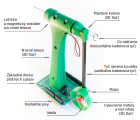
\includegraphics{AS_parts_foto.pdf}
        }

        \figcaption{
            % Signály systému \emph{AS}.
        }
        \label{AS_parts_foto}
    }%vbox

    \vspace{-6pt}

\end{figure}

Konštrukcia kyvadla zariadenia je tvorená horizontálnou a vertikálnou karbónovou tyčou, ktoré sú spojené plastovým komponentom realizovaným 3D tlačou. Horizontálna tyč je hriadeľom v osi otáčania kyvadla a vertikálna tyč je ramenom kyvadla. Na konci ramena je upevnený malý jednosmerný motor s vrtuľou čím je realizovaný pohon kyvadla schopný ho vychýliť. Napájanie motora je spínané tranzistorom. Na konci otáčajúceho sa hriadeľa je pripevnený magnet ako súčasť rotačného magnetického enkódera realizujúceho snímanie uhla natočenia ramena kyvadla. Encoder poskytuje informáciu o uhle prostredníctvom komunikačného rozhrania I$2$C.

Súčasťou zariadenia je aj potenciometer, ktorý vo všeobecnosti umožňuje realizovať manuálny napäťový signál.

Používanie opísaného zariadenia predpokladá:

\begin{itemize}[leftmargin=0pt, labelsep=3mm, itemsep=0pt]
    \item Spínanie tranzistora na napájanie motora -- typicky v zmysle PWM signálu (angl. Pulse-Width Modulation). Hradlo tranzistora (gate) je pripojené na pin D$5$.
    \item Čítanie informácie o uhle natočenia ramena kyvadla prostredníctvom I$2$C rozhrania. Pripojené na pinoch SDA a SCL.
    \item Snímanie napätia potenciometra ktorého bežec je pripojený na pin A$0$.
\end{itemize}



\subsubsection{Softvér}

Pre zariadenia AutomationShield ako celok je dostupná softvérová knižnica realizujúca C/C++~API. Podknižnica pre AeroShield je súčasťou tejto knižnice a poskytuje jednoduché rozhranie pre prácu so zariadením. Knižnica zabezpečuje inicializáciu zariadenia a prístup k jeho vstupom a výstupom. Pre ilustráciu:

% \begin{lstlisting}[language=C++, caption={Ukážky použitia funkcionality knižnice AeroShield, ktorá je súčasťou balíka AutomationShield.}]
\begin{lstlisting}[language=C++]
#include <AeroShield.h>

//... iný kód ...

void setup()
{
	AeroShield.begin();
	AeroShield.calibrate();

    //... iný kód ...
}

void loop()
{
    //... iný kód ...

    // nastavenie vstup. signálu (napájanie motora)
    AeroShield.actuatorWrite(u);  

    // čítanie výstup. signálu (uhol)
    y = AeroShield.sensorRead();  

    // čítanie signálu z potenciometra
    r = AeroShield.referenceRead(); 

    //... iný kód ...
}
\end{lstlisting}
Vyžaduje sa pritom, aby hodnota vstupného signálu bola desatinné číslo v rozsahu $0,0$ až $100,0$, predstavuje 0 až 100 percent napájacieho napätia motora. Výstupný signál je desatinné číslo, ktoré je priamo hodnotou uhla v stupňoch (vyžaduje si to korektnú inicializáciu a kalibráciu zariadenia). Signál z potenciometra je desatinné číslo v rozsahu $0,0$ až $100,0$, predstavujúce 0 až 100 percent pozície potenciometra.


\paragraph{Referencie}

\begin{itemize}[leftmargin=0pt, labelsep=3mm, itemsep=0pt]
    \item GitHub wiki: {\scriptsize \url{https://github.com/gergelytakacs/AutomationShield/wiki/AeroShield}}
\end{itemize}



\section{Opis dynamického systému}


Zariadenie AeroShield je z hľadiska opisu dynamického systému kyvadlo s pohonom. Pohon je realizovaný ťahom (ťahom vzduchu) vrtule umiestnenej na konci ramena kyvadla. Zariadenie pozostáva so základnej dosky plošných spojov, nosného telesa kyvadla a samotného ramena kyvadla. Na doske plošných spojov sú elektronické obvody realizujúce napájanie zariadenia a rozhranie na úrovni elektrických signálov.

Z celkového hľadiska má systém jeden vstupný signál a jeden výstupný signál. Vstup je vo forme PWM signálu, ktorý ovláda napájanie elektrického motora poháňajúceho vrtuľu. Výstup je vo forme digitálnych dát na I$2$C zbernici integrovaného obvodu obsahujúceho rotačný magnetický enkóder, ktorý sníma uhol natočenia ramena kyvadla. Zariadenie obsahuje aj potenciometer ako napäťový delič a tento napäťový signál je dostupný pre používateľa pre rôzne využitie (manuálne nastaviteľný signál).




\section{Rozsahy a jednotky signálov}

Predpokladáme, že hardvér a softvér realizujúci opísaný dynamický systém sú ako v~časti~\ref{AutomationShieldDescription}. Potom z opisu systému vyplýva, že systém ma jeden vstupný signál, jeden výstupný signál a manuálne nastaviteľný signál.

Vstupný signál nadobúda hodnoty v rozsahu $0$ až $100$, pričom ide o veľkosť striedy (duty cycle) PWM signálu v percentách [\%]. 

Výstupný signál je hodnota uhla natočenia ramena kyvadla v stupňoch [\si{\degree}]. Predpokladá sa, že inicializácia a kalibrácia zariadenia prebiehajú keď je rameno v pokoji a základná doska (plošných spojov) je vodorovná. Táto poloha je označená ako \ang{0}. Rameno kyvadla má fyzické dorazy obmedzujúce jeho natočenie a za uvedeného predpokladu tieto dorazy umožňujú natočenie ramena v rozsahu približne \ang{-60} až \ang{210}. 

Manuálne nastaviteľný napäťový signál potenciometra, ktorý je spracovaný uvedenou softvérovou knižnicou, nadobúda hodnoty v rozsahu $0$ až $100$ v percentách [\%]. Reprezentuje fyzickú pozíciu bežca potenciometra.


\begin{center}

\vspace{-10pt}    
    
\tabcaption{Rozsahy a jednotky signálov}
\label{tab:rozsahy_a_jednotky_signalu}

\lstyle

\begin{tabular*}{\textwidth}{@{ \extracolsep{\fill}} lll}
\toprule
Signál & Rozsah hodnôt & Jednotka \\
\midrule
Vstup & $0$ až $100$ & \% (percento) \\
Výstup & $-60$ až $210$ & \si{\degree} (stupeň) \\
Potenciometer & $0$ až $100$ & \% (percento) \\
\bottomrule
\end{tabular*}

\end{center}











\section{Schematické znázornenie systému}


\begin{center}

    \vbox{%


        \makebox[\textwidth][c]{%
            % \includegraphics{SystemSchemeBase.pdf}
            \begin{tikzpicture}

                \node[block, align=center] (plant) {Systém\\AeroShield};
                \node[left=2cm of plant] (input_node) {};
                \node[right=2cm of plant, shift={(0,0.5cm)}] (output_node) {};
                \node[right=2cm of plant, shift={(0,-0.5cm)}] (pot_node) {};


                \draw[line] (input_node) -- (plant)
                    node[midway, above, align=center] {Vstup\\$0 \text{ - } 100$ \%};

                \draw [line] ($(plant.east)+(0,0.5cm)$) -- (output_node)
                    node[midway,above,align=center] {Výstup\\$-60 \text{ - } 210$ [$^\circ$]};

                \draw [line] ($(plant.east)+(0,-0.5cm)$) -- (pot_node)
                    node[midway,above,align=center] {Potenciometer\\$0 \text{ - } 100$ [\%]};


            \end{tikzpicture}
        }

        \figcaption{
            Signály systému AeroShield.
        }
        \label{AS_scheme}
    }%vbox

\end{center}

















% -----------------------------------------------------------------------------

\end{document}

% -----------------------------------------------------------------------------